% move all configuration stuff into includes file so we can focus on the content
\documentclass[aspectratio=169,hyperref={pdfpagelabels=false,colorlinks=true,linkcolor=white,urlcolor=blue},t]{beamer}

%%%%%%%%%%%%%%%%%%%%%%%%%%%%%%%%%%%%%%%%%%%%%%%%%%%%%%%%%%%%%%%%%%%%%%%%%%%%%%%%%%
%%%%%%%%%%%%%%%%%%%%%%%%%%%%%%%%%%%%%%%%%%%%%%%%%%%%%%%%%%%%%%%%%%%%%%%%%%%%%%%%%%
% packages
\usepackage{pict2e}
\usepackage{epic}
\usepackage{amsmath,amsfonts,amssymb}
\usepackage{units}
\usepackage{fancybox}
\usepackage[absolute,overlay]{textpos} 
\usepackage{media9} % avi2flv: "C:\Program Files\ffmpeg\bin\ffmpeg.exe" -i TuneFreqFilterbank.avi -b 600k -s 441x324 -r 15 -acodec copy TuneFreqFilterbank.flv
\usepackage{animate}
\usepackage{gensymb}
\usepackage{multirow}
\usepackage{silence}
\usepackage{tikz}
\usepackage[backend=bibtex,style=ieee]{biblatex}
\AtEveryCitekey{\iffootnote{\tiny}{}}
\addbibresource{include/references}

%%%%%%%%%%%%%%%%%%%%%%%%%%%%%%%%%%%%%%%%%%%%%%%%%%%%%%%%%%%%%%%%%%%%%%%%%%%%%%%%%%
%%%%%%%%%%%%%%%%%%%%%%%%%%%%%%%%%%%%%%%%%%%%%%%%%%%%%%%%%%%%%%%%%%%%%%%%%%%%%%%%%%
% relative paths
\graphicspath{{graph/}}


%%%%%%%%%%%%%%%%%%%%%%%%%%%%%%%%%%%%%%%%%%%%%%%%%%%%%%%%%%%%%%%%%%%%%%%%%%%%%%%%%%
%%%%%%%%%%%%%%%%%%%%%%%%%%%%%%%%%%%%%%%%%%%%%%%%%%%%%%%%%%%%%%%%%%%%%%%%%%%%%%%%%%
% units
\setlength{\unitlength}{1mm}

%%%%%%%%%%%%%%%%%%%%%%%%%%%%%%%%%%%%%%%%%%%%%%%%%%%%%%%%%%%%%%%%%%%%%%%%%%%%%%%%%%
%%%%%%%%%%%%%%%%%%%%%%%%%%%%%%%%%%%%%%%%%%%%%%%%%%%%%%%%%%%%%%%%%%%%%%%%%%%%%%%%%%
% theme & layout
\usetheme{Frankfurt}
\beamertemplatenavigationsymbolsempty
%\setbeamertemplate{frametitle}[smoothbars theme]
\setbeamertemplate{frametitle}
{
    \begin{beamercolorbox}[ht=1.8em,wd=\paperwidth]{frametitle}
        \vspace{-.1em}%
        \hspace{.2em}{\strut\insertframetitle\strut}
        
        \hspace{.2em}\small\strut\insertframesubtitle\strut
        %\hfill
        %\includegraphics[height=.8cm,keepaspectratio]{CenterMusicTechnology-solid-2lines-white-CoAtag}
        
    \end{beamercolorbox}
    \begin{textblock*}{100mm}(11.6cm,.7cm)
        \includegraphics[height=.8cm,keepaspectratio]{Logo_GTCMT_black}
    \end{textblock*}
}
\setbeamertemplate{footline}[frame number]

% set this to ensure bulletpoints without subsections
\usepackage{remreset}
\makeatletter
\@removefromreset{subsection}{section}
\makeatother
\setcounter{subsection}{1}

%---------------------------------------------------------------------------------
% appearance
\setbeamercolor{structure}{fg=gtgold}
\setbeamercovered{transparent} %invisible
\setbeamercolor{bibliography entry author}{fg=black}
\setbeamercolor*{bibliography entry title}{fg=black}
\setbeamercolor*{bibliography entry note}{fg=black}
\setbeamercolor{frametitle}{fg=black}
\setbeamercolor{title}{fg=black}

%\usepackage{pgfpages}
%\setbeameroption{show notes}
%\setbeameroption{show notes on second screen=right}
%---------------------------------------------------------------------------------
% fontsize
\let\Tiny=\tiny

%%%%%%%%%%%%%%%%%%%%%%%%%%%%%%%%%%%%%%%%%%%%%%%%%%%%%%%%%%%%%%%%%%%%%%%%%%%%%%%%%%
%%%%%%%%%%%%%%%%%%%%%%%%%%%%%%%%%%%%%%%%%%%%%%%%%%%%%%%%%%%%%%%%%%%%%%%%%%%%%%%%%%
% warnings
\pdfsuppresswarningpagegroup=1
\WarningFilter{biblatex}{Patching footnotes failed}
\WarningFilter{latexfont}{Font shape}
\WarningFilter{latexfont}{Some font shapes}
\WarningFilter{gensymb}{Not defining}


%%%%%%%%%%%%%%%%%%%%%%%%%%%%%%%%%%%%%%%%%%%%%%%%%%%%%%%%%%%%%%%%%%%%%%%%%%%%%%%%%%
%%%%%%%%%%%%%%%%%%%%%%%%%%%%%%%%%%%%%%%%%%%%%%%%%%%%%%%%%%%%%%%%%%%%%%%%%%%%%%%%%%
% theme & layout
\usetheme{Frankfurt}
\useinnertheme{rectangles}


%%%%%%%%%%%%%%%%%%%%%%%%%%%%%%%%%%%%%%%%%%%%%%%%%%%%%%%%%%%%%%%%%%%%%%%%%%%%%%%%%%
\setbeamertemplate{frametitle}[default][colsep=-4bp,rounded=false,shadow=false]
\setbeamertemplate{frametitle}
{%
    \nointerlineskip%
    %\vskip-0.5ex
    \begin{beamercolorbox}[wd=\paperwidth,ht=3.5ex,dp=0.6ex]{frametitle}
        \hspace*{1.3ex}\insertframetitle%
        
        \hspace*{1.3ex}\small\insertframesubtitle%
    \end{beamercolorbox}%
    \begin{textblock*}{100mm}(11.6cm,.57cm)
        
\includegraphics[height=.8cm,keepaspectratio]{graph/Logo_GTCMT_white}
    \end{textblock*}
}


%%%%%%%%%%%%%%%%%%%%%%%%%%%%%%%%%%%%%%%%%%%%%%%%%%%%%%%%%%%%%%%%%%%%%%%%%%%%%%%%%%
\setbeamertemplate{title page}[default][colsep=-4bp,rounded=false,shadow=false]
\setbeamertemplate{title page}
{
    \begin{textblock*}{100mm}(15cm,.51cm)
            \href{https://github.com/alexanderlerch/ACA-Slides/blob/2nd_edition/\jobname.pdf}{\includegraphics[height=.5cm,keepaspectratio]{graph/Logo_github}}\hspace*{2ex}
    \end{textblock*}
    \vskip-10ex
    \begin{beamercolorbox}[wd=\paperwidth,ht=.7\paperheight,dp=0.6ex]{frametitle} %35ex
        %\begin{flushright}
            %\href{http://www.gtcmt.gatech.edu}{\includegraphics[height=.8cm,keepaspectratio]{graph/Logo_GTCMT_black}}\hspace*{2ex}
        %\end{flushright}
        
        \hspace*{1.8ex}\LARGE\inserttitle%
        
        \vspace*{.5ex}
        
        \hspace*{1.3ex}\small\insertsubtitle%
        
        \vspace*{.5ex}
    \end{beamercolorbox}%
    \nointerlineskip%
    \begin{beamercolorbox}[wd=\paperwidth,ht=.4\paperheight,dp=0.6ex]{page number in head/foot}
        %\vspace*{-.5ex}
        \hspace*{1.7ex}\small\insertauthor%
        
        %\hspace*{1.7ex}\small }%
        
        \vspace*{10ex}
        
        \begin{flushright}
            \href{http://www.gtcmt.gatech.edu}{\includegraphics[height=.8cm,keepaspectratio]{graph/Logo_GTCMT_black}}\hspace*{2ex}
        \end{flushright}
    \end{beamercolorbox}%
}


%%%%%%%%%%%%%%%%%%%%%%%%%%%%%%%%%%%%%%%%%%%%%%%%%%%%%%%%%%%%%%%%%%%%%%%%%%%%%%%%%%
%\makeatother
\setbeamertemplate{footline}
{
  \leavevmode%
  \hbox{%
  \begin{beamercolorbox}[wd=.5\paperwidth,ht=2.25ex,dp=1ex,left,leftskip=1ex]{page number in head/foot}%
    \insertsubtitle
  \end{beamercolorbox}%
  \begin{beamercolorbox}[wd=.5\paperwidth,ht=2.25ex,dp=1ex,right,rightskip=1ex]{page number in head/foot}%
    \hfill
    \insertframenumber{} / \inserttotalframenumber
  \end{beamercolorbox}}%
  \vskip0pt%
}
%\makeatletter


%%%%%%%%%%%%%%%%%%%%%%%%%%%%%%%%%%%%%%%%%%%%%%%%%%%%%%%%%%%%%%%%%%%%%%%%%%%%%%%%%%
\beamertemplatenavigationsymbolsempty
\setbeamertemplate{navigation symbols}{}
\setbeamertemplate{blocks}[default]%[rounded=false,shadow=false]
\setbeamertemplate{itemize item}[square]
\setbeamertemplate{itemize subitem}[circle]
\setbeamertemplate{itemize subsubitem}[triangle]
\setbeamertemplate{enumerate item}[square]
\setbeamertemplate{enumerate subitem}[circle]
\setbeamertemplate{enumerate subsubitem}[circle]


%%%%%%%%%%%%%%%%%%%%%%%%%%%%%%%%%%%%%%%%%%%%%%%%%%%%%%%%%%%%%%%%%%%%%%%%%%%%%%%%%%
% colors
\setbeamercolor{structure}{fg=darkgray}
\setbeamercovered{transparent} %invisible
\setbeamercolor{bibliography entry author}{fg=black}
\setbeamercolor*{bibliography entry title}{fg=black}
\setbeamercolor*{bibliography entry note}{fg=black}
\setbeamercolor{frametitle}{fg=black}
\setbeamercolor{title}{fg=white}
\setbeamercolor{subtitle}{fg=white}
\setbeamercolor{frametitle}{fg=white}
\setbeamercolor{framesubtitle}{fg=white}
\setbeamercolor{mini frame}{fg=white, bg=black}
\setbeamercolor{section in head/foot}{fg=white, bg=darkgray}
\setbeamercolor{page number in head/foot}{fg=black, bg=lightblue}
\setbeamercolor{item projected}{fg=white, bg=black}

%---------------------------------------------------------------------------------
%%%%%%%%%%%%%%%%%%%%%%%%%%%%%%%%%%%%%%%%%%%%%%%%%%%%%%%%%%%%%%%%%%%%%%%%%%%%%%%%%%
%%%%%%%%%%%%%%%%%%%%%%%%%%%%%%%%%%%%%%%%%%%%%%%%%%%%%%%%%%%%%%%%%%%%%%%%%%%%%%%%%%
% title information
\title[]{Introduction to \textbf{Audio Content Analysis}}   
\author[alexander lerch]{alexander lerch} 
%\institute{~}
%\date[Alexander Lerch]{}
%\titlegraphic{\vspace{-16mm}\includegraphics[width=\textwidth,height=3cm]{title}}

%%%%%%%%%%%%%%%%%%%%%%%%%%%%%%%%%%%%%%%%%%%%%%%%%%%%%%%%%%%%%%%%%%%%%%%%%%%%%%%%%%
%%%%%%%%%%%%%%%%%%%%%%%%%%%%%%%%%%%%%%%%%%%%%%%%%%%%%%%%%%%%%%%%%%%%%%%%%%%%%%%%%%
% colors
\definecolor{gtgold}{HTML}{E0AA0F} %{rgb}{0.88,0.66,1,0.06} [234, 170, 0]/256
\definecolor{darkgray}{rgb}{.1, .1, .25}
\definecolor{lightblue}{rgb}{.1, 0.75, 1}
\definecolor{highlight}{rgb}{0, 0, 1} %_less!40

%%%%%%%%%%%%%%%%%%%%%%%%%%%%%%%%%%%%%%%%%%%%%%%%%%%%%%%%%%%%%%%%%%%%%%%%%%%%%%%%%%
%%%%%%%%%%%%%%%%%%%%%%%%%%%%%%%%%%%%%%%%%%%%%%%%%%%%%%%%%%%%%%%%%%%%%%%%%%%%%%%%%%
% relative paths
\graphicspath{{../ACA-Plots/graph/}}


%%%%%%%%%%%%%%%%%%%%%%%%%%%%%%%%%%%%%%%%%%%%%%%%%%%%%%%%%%%%%%%%%%%%%%%%%%%%%%%%%%
%%%%%%%%%%%%%%%%%%%%%%%%%%%%%%%%%%%%%%%%%%%%%%%%%%%%%%%%%%%%%%%%%%%%%%%%%%%%%%%%%%
% units
\setlength{\unitlength}{1mm}

%%%%%%%%%%%%%%%%%%%%%%%%%%%%%%%%%%%%%%%%%%%%%%%%%%%%%%%%%%%%%%%%%%%%%%%%%%%%%%%%%%
%%%%%%%%%%%%%%%%%%%%%%%%%%%%%%%%%%%%%%%%%%%%%%%%%%%%%%%%%%%%%%%%%%%%%%%%%%%%%%%%%%
% math
\DeclareMathOperator*{\argmax}{argmax}
\DeclareMathOperator*{\argmin}{argmin}
\DeclareMathOperator*{\atan}{atan}
\DeclareMathOperator*{\arcsinh}{arcsinh}
\DeclareMathOperator*{\sign}{sign}
\DeclareMathOperator*{\tcdf}{tcdf}
\DeclareMathOperator*{\si}{sinc}
\DeclareMathOperator*{\princarg}{princarg}
\DeclareMathOperator*{\arccosh}{arccosh}
\DeclareMathOperator*{\hwr}{HWR}
\DeclareMathOperator*{\flip}{flip}
\DeclareMathOperator*{\sinc}{sinc}
\DeclareMathOperator*{\floor}{floor}
\newcommand{\e}{{e}}
\newcommand{\jom}{\mathrm{j}\omega}
\newcommand{\jOm}{\mathrm{j}\Omega}
\newcommand   {\mat}[1]    		{\boldsymbol{\uppercase{#1}}}		%bold
\renewcommand {\vec}[1]    		{\boldsymbol{\lowercase{#1}}}		%bold

%%%%%%%%%%%%%%%%%%%%%%%%%%%%%%%%%%%%%%%%%%%%%%%%%%%%%%%%%%%%%%%%%%%%%%%%%%%%%%%%%%
%%%%%%%%%%%%%%%%%%%%%%%%%%%%%%%%%%%%%%%%%%%%%%%%%%%%%%%%%%%%%%%%%%%%%%%%%%%%%%%%%%
% media9
\newcommand{\includeaudio}[1]{
\href{run:audio/#1.mp3}{
\includegraphics[width=5mm, height=5mm]{graph/SpeakerIcon}}}

\newcommand{\includeanimation}[4]{{\begin{center}
                        \animategraphics[autoplay,loop,scale=.7]{#4}{animation/#1-}{#2}{#3}        
                        \end{center}
                        \addreference{matlab source: \href{https://github.com/alexanderlerch/ACA-Plots/blob/master/matlab/animate#1.m}{matlab/animate#1.m}}}
                        \inserticon{video}}
                        
%%%%%%%%%%%%%%%%%%%%%%%%%%%%%%%%%%%%%%%%%%%%%%%%%%%%%%%%%%%%%%%%%%%%%%%%%%%%%%%%%%
%%%%%%%%%%%%%%%%%%%%%%%%%%%%%%%%%%%%%%%%%%%%%%%%%%%%%%%%%%%%%%%%%%%%%%%%%%%%%%%%%%
% other commands
\newcommand{\question}[1]{%\vspace{-4mm}
                          \setbeamercovered{invisible}
                          \begin{columns}[T]
                            \column{.9\textwidth}
                                \textbf{#1}
                            \column{.1\textwidth}
                                \vspace{-8mm}
                                \begin{flushright}
                                     
\includegraphics[width=.9\columnwidth]{graph/question_mark}
                                \end{flushright}
                                \vspace{6mm}
                          \end{columns}\pause\vspace{-12mm}}

\newcommand{\toremember}[1]{
                        \inserticon{lightbulb}
                        }

\newcommand{\matlabexercise}[1]{%\vspace{-4mm}
                          \setbeamercovered{invisible}
                          \begin{columns}[T]
                            \column{.8\textwidth}
                                \textbf{matlab exercise}: #1
                            \column{.2\textwidth}
                                \begin{flushright}
                                     \includegraphics[scale=.5]{graph/logo_matlab}
                                \end{flushright}
                                %\vspace{6mm}
                          \end{columns}}

\newcommand{\addreference}[1]{  
                  
                    \begin{textblock*}{\baselineskip }(.98\paperwidth,.5\textheight) %(1.15\textwidth,.4\textheight)
                         \begin{minipage}[b][.5\paperheight][b]{1cm}%
                            \vfill%
                             \rotatebox{90}{\tiny {#1}}
                        \end{minipage}
                   \end{textblock*}
                    }
                    
\newcommand{\figwithmatlab}[1]{
                    \begin{figure}
                        \centering
                        \includegraphics[scale=.7]{#1}
                        %\label{fig:#1}
                    \end{figure}
                    
                    \addreference{matlab source: \href{https://github.com/alexanderlerch/ACA-Plots/blob/main/matlab/plot#1.m}{plot#1.m}}}
\newcommand{\figwithref}[2]{
                    \begin{figure}
                        \centering
                        \includegraphics[scale=.7]{#1}
                        \label{fig:#1}
                    \end{figure}
                    
                    \addreference{#2}}  
                                    
\newcommand{\inserticon}[1]{
                    \begin{textblock*}{100mm}(14.5cm,7.5cm)
                        \includegraphics[height=.8cm,keepaspectratio]{graph/#1}
                    \end{textblock*}}            

%%%%%%%%%%%%%%%%%%%%%%%%%%%%%%%%%%%%%%%%%%%%%%%%%%%%%%%%%%%%%%%%%%%%%%%%%%%%%%%%%%
%%%%%%%%%%%%%%%%%%%%%%%%%%%%%%%%%%%%%%%%%%%%%%%%%%%%%%%%%%%%%%%%%%%%%%%%%%%%%%%%%%
% counters
\newcounter{i}
\newcounter{j}
\newcounter{iXOffset}
\newcounter{iYOffset}
\newcounter{iXBlockSize}
\newcounter{iYBlockSize}
\newcounter{iYBlockSizeDiv2}
\newcounter{iXBlockSizeDiv2}
\newcounter{iDistance}




\subtitle{Module 4.1: Classification}

%%%%%%%%%%%%%%%%%%%%%%%%%%%%%%%%%%%%%%%%%%%%%%%%%%%%%%%%%%%%%%%%%%%%%%%%%%%%
\begin{document}
    % generate title page
	{
\setbeamertemplate{headline}{} 
\setbeamertemplate{footline}{} 
\begin{frame}
    \titlepage
    %\vspace{-5mm}
\end{frame}
}
\addtocounter{framenumber}{-1}


    \section[overview]{lecture overview}
        \begin{frame}{introduction}{overview}
            \begin{block}{corresponding textbook section}
                    %\href{http://ieeexplore.ieee.org/xpl/articleDetails.jsp?arnumber=6331125}{Chapter 8: Musical Genre, Similarity, and Mood} (pp.~155)
                    Section~4.1
            \end{block}

            \begin{itemize}
                \item   \textbf{lecture content}
                    \begin{itemize}
                        \item   intuitive intro to machine learning
                        \item   classifier examples
                    \end{itemize}
                \bigskip
                \item<2->   \textbf{learning objectives}
                    \begin{itemize}
                        \item   describe the basic principles of data-driven machine learning approaches
                        \item   implement a kNN classifier in Python
                    \end{itemize}
            \end{itemize}
            \inserticon{directions}
        \end{frame}

    \section[intro]{introduction}
        \begin{frame}{classification}{introduction}
            remember the flow chart of a general ACA system:
            \vspace{-3mm}
            \begin{figure}
                \begin{footnotesize}
				\begin{picture}(96,26)
					\setcounter{iXOffset}{0}
					\setcounter{iYOffset}{5}
					\setcounter{iXBlockSize}{28}
					\setcounter{iYBlockSize}{16}
					\setcounter{iYBlockSizeDiv2}{8}
					\setcounter{iDistance}{8}
	
					\addtocounter{iYOffset}{\value{iYBlockSizeDiv2}}
					\addtocounter{iYOffset}{-2}
	
					%\addtocounter{iXOffset}{-1}
					\put(\value{iXOffset}, \value{iYOffset})
						{\text{{\shortstack[c]{audio\\ signal}}}}
					\addtocounter{iXOffset}{1}
	
					\addtocounter{iYOffset}{2}
					\addtocounter{iXOffset}{\value{iDistance}}
	
					\put(\value{iXOffset}, \value{iYOffset})
						{\vector(1,0){\value{iDistance}}}
	
					\addtocounter{iXOffset}{\value{iDistance}}
					\addtocounter{iYOffset}{-\value{iYBlockSizeDiv2}}
					
					\put(\value{iXOffset}, \value{iYOffset})
						{\framebox(\value{iXBlockSize}, \value{iYBlockSize}) {\shortstack[c]{feature\\ extraction}}}
	
					\addtocounter{iXOffset}{\value{iXBlockSize}}
					\addtocounter{iYOffset}{\value{iYBlockSizeDiv2}}
	
					\put(\value{iXOffset}, \value{iYOffset})
						{\vector(1,0){\value{iDistance}}}
	
					\addtocounter{iXOffset}{\value{iDistance}}
					\addtocounter{iYOffset}{-\value{iYBlockSizeDiv2}}
	
					\put(\value{iXOffset}, \value{iYOffset})
						{\framebox(\value{iXBlockSize}, \value{iYBlockSize}) {\color{highlight}{\shortstack[c]{decision,\\ interpretation,\\ classification,\\ inference}}}}
	
					\addtocounter{iXOffset}{\value{iXBlockSize}}
					\addtocounter{iYOffset}{\value{iYBlockSizeDiv2}}
	
					\put(\value{iXOffset}, \value{iYOffset})
						{\vector(1,0){\value{iDistance}}}
	
					\addtocounter{iXOffset}{\value{iDistance}}
					\addtocounter{iYOffset}{-2}
	
					\addtocounter{iXOffset}{1}
					\put(\value{iXOffset}, \value{iYOffset})
						{\text{{\shortstack[c]{meta\\ data}}}}
					
				\end{picture}
\end{footnotesize}

            \end{figure}
            \begin{itemize}
                \item<2->   \color<3->{gtgold}{\textit{classification}}: 
                    \begin{itemize}
                        \item   assign class labels to data
                    \end{itemize}
                \item<2->   \textit{regression}:
                    \begin{itemize}
                        \item	estimate numerical labels for data
                    \end{itemize}
                \item<2->   \textit{clustering}:
                    \begin{itemize}
                        \item	find grouping patterns in data
                    \end{itemize}
            \end{itemize}
        \end{frame}
        \begin{frame}{classification}{basic example}
              %\vspace{-3mm}
             \begin{columns}
                \column{.4\linewidth} 
                    hypothetical system:
                    \begin{itemize}
                        \item   one feature (envelope)
                        \item   predefined threshold
                            \begin{itemize}
                                \item   higher than threshold\\ $\Rightarrow$ class 1 (onset)
                                \item   lower than threshold\\ $\Rightarrow$ class 0 (no onset)
                            \end{itemize}
                    \end{itemize}
                \column{.6\linewidth} 
                \vspace{-10mm}
                            \figwithmatlab{ThresholdClassification}
            \end{columns}
        \end{frame}
        
        \begin{frame}{classification}{data-driven}
             \vspace{-3mm}
             \begin{columns}
                \column{.4\linewidth} 
                   \begin{itemize}
                        \item   derive classification parameters from data, e.g.,
                        \item[$\Rightarrow$]  learn common feature distributions per class
                        \item[$\Rightarrow$]  learn separation metrics per class
                    \end{itemize}
                \column{.6\linewidth} 
                \vspace{-10mm}
                    \figwithmatlab{FeatureSpace}
            \end{columns}
        \end{frame}
        
        %\begin{frame}{classification}{general steps}
            %\begin{enumerate}
                %\item	\textbf{define training set}: annotated results
                %\smallskip
                %\item<2->	\textbf{normalize} training set
                %\smallskip
                %\item<3->	\textbf{train} classifier
                %\smallskip
                %\item<4->	\textbf{evaluate} classifier with test (or validation) set
                %\smallskip
                %\item<5->	(\textbf{adjust} classifier settings, return to 4.)
            %\end{enumerate}
        %\end{frame}
        %
    %\section{classification}
        %\begin{frame}{classification}{rules of thumb}
            %\vspace{-3mm}
            %\begin{itemize}
                %\item   \textbf{training set}
                    %\begin{itemize}
                        %\item	training set size vs.\ number of features
                            %\begin{itemize}
                                %\item	training set too small,% $\Rightarrow$ \textit{overfitting}
                                %feature number too large $\Rightarrow$ \textit{overfitting}
                            %\end{itemize}
                        %\item<1->	training set \textbf{too noisy} $\Rightarrow$ \textit{underfitting}
                        %\item<1->	training set \textbf{not representative} $\Rightarrow$ \textit{bad classification performance}
                    %\end{itemize}
                %\smallskip
                %\item<2->   \textbf{classifier}
                    %\begin{itemize}
                        %\item<2->   classifier too complex $\Rightarrow$ \textit{overfitting}
                        %\item<2->	\textbf{poor classifier} $\Rightarrow$ \textit{bad classification performance}
                            %\begin{itemize}
                                %\item[$\rightarrow$]	different classifier
                            %\end{itemize}
                    %\end{itemize}
                %\smallskip
                %\item<3->   \textbf{features}
                    %\begin{itemize}
                        %\item<3->	\textbf{poor features} $\Rightarrow$ \textit{bad classification performance}
                            %\begin{itemize}
                                %\item[$\rightarrow$]	new, better features
                            %\end{itemize}
                        %\item<3->	features \textbf{not normalized} $\Rightarrow$ possibly \textit{bad classification performance}
                            %\begin{itemize}
                                %\item	feature distribution (range, mean, symmetry)
                            %\end{itemize}
                    %\end{itemize}
            %\end{itemize}
        %\end{frame}
        %\begin{frame}{classification}{evaluation}
            %\begin{itemize}
                %\item	define \textbf{test set} for evaluation
                    %\begin{itemize}
                        %\item	test set \textit{different} from training set
                        %\item	otherwise, same requirements
                    %\end{itemize}
                %
                %\bigskip
                %\item<2->	example: \textbf{$N$-fold cross validation}
                    %\begin{enumerate}
                        %\item<2->	split training set into $N$ parts (randomly, but preferably identical number per class)
                        %\item<3->	select one part as test set
                        %\item<4->	train the classifier with all observations from remaining $N-1$ parts
                        %\item<5->	compute the classification rate for the test set
                        %\item<6->	repeat until all $N$ parts have been tested
                        %\item<7->	overall result: \textit{average} classification rate
                    %\end{enumerate}
            %\end{itemize}
        %\end{frame}
        %
     \section[examples]{classifier examples}
        \begin{frame}{classifier examples}{k-Nearest Neighbor (kNN)}
            \begin{columns}
                \column{.6\linewidth} 
                    \begin{itemize}
                        \item	\textbf{training}: extract reference vectors from training set 
                            \begin{itemize}
                                \item store coordinates and class labels
                            \end{itemize}
                        \item<2->	\textbf{classification}: extract query vector and set class to majority of $k$ nearest reference vectors
                            \begin{enumerate}
                                \item   compute distance between query and all training vectors
                                \item   sort distances to find closest vectors
                                \item   choose majority class out of the $k$ closest vectors
                            \end{enumerate}
                        \bigskip
                        \item<3->	\textbf{classifier model}: all training vectors
                    \end{itemize}
                \column{.4\linewidth} 
                    %\only<1,6>{\begin{figure}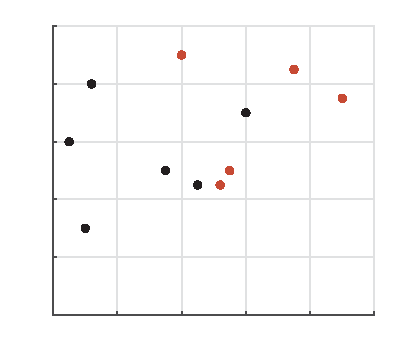
\includegraphics[width=\columnwidth]{Knn-0}\end{figure}}
                    %\setcounter{i}{1}
                    %\setcounter{j}{2}
                    %\whiledo{\value{i}<5}
                    %{
                        %\only<\value{j}>{\begin{figure}\includegraphics[width=\columnwidth]{Knn-\arabic{i}}\end{figure}}
                        %\stepcounter{i}
                        %\stepcounter{j}
                    %}
                    \figwithmatlab{Knn}
                    \only<4>{$k = 3 \Rightarrow$ gold majority}
                    \only<5>{$k = 5 \Rightarrow$ black majority}
                    \only<6>{$k = 7 \Rightarrow$ black majority}
            \end{columns}
        \end{frame}
        \begin{frame}{classifier examples}{Gaussian Mixture Model (GMM)}
            \vspace{-3mm}
             \begin{columns}
                \column{.4\linewidth} 
                   \begin{itemize}
                        \item	\textbf{training}:\\ model each class distribution as superposition of Gaussian distributions
                        \item<2->	\textbf{classification}:\\ compute output of each Gaussian and select class with highest probability
                        \item<3->	\textbf{classifier data}:\\ per class per Gaussian: $\mu$ and covariance, mixture weight
                    \end{itemize}
                \column{.6\linewidth} 
                \vspace{-13mm}
                    \figwithmatlab{Gmm}
            \end{columns}
        \end{frame}
        \begin{frame}{classifier examples}{Support Vector Machine (SVM)}
            \begin{itemize}
                \item	\textbf{training}:
                    \begin{itemize}
                        \item   map features to high dimensional space
                            \figwithref{graph/SVM}{\href{https://en.wikipedia.org/wiki/Support\_vector\_machine}{https://en.wikipedia.org/wiki/Support\_vector\_machine}}
                        \item   find separating hyperplane through maximum distance of support vectors (data points)
                    \end{itemize}
                \item<2->	\textbf{classification}: apply feature transform and proceed with 'linear' classification
                \item<3->	\textbf{classifier data}: support vectors, kernel, kernel parameters
            \end{itemize}
        \end{frame}
    
    \section{summary}
        \begin{frame}{summary}{lecture content}
            \begin{itemize}
                \item   \textbf{data-driven approach}
                    \begin{itemize}
                        \item   'general' system learns parameters/behavior from data
                        \item   human interaction through
                            \begin{itemize}
                                \item   parametrization and procedures
                                \item   data selection
                            \end{itemize}
                    \end{itemize}
                \bigskip
                \item   \textbf{many classifiers with different levels of complexity}
                    \begin{enumerate}
                        \item   kNN
                        \item   GMM
                        \item   SVM
                        \item   RandomForest
                        \item   DNN
                        \item   \ldots
                    \end{enumerate}
                %\bigskip
                %\item   \textbf{fine balance of inputs}
                    %\begin{enumerate}
                        %\item   number of features
                        %\item   classifier complexity
                        %\item   amount and variability of data
                    %\end{enumerate}
            \end{itemize}
            \inserticon{summary}
        \end{frame}
\end{document}
